%----------------------------------------------------------------------------------------
%	PACKAGES AND OTHER DOCUMENT CONFIGURATIONS
%----------------------------------------------------------------------------------------

\documentclass[fleqn,10pt]{article} % Document font size and equations flushed left

\setcounter{tocdepth}{3} % Show only three levels in the table of contents section: sections, subsections and subsubsections


% Pandoc environments
\usepackage{framed}
\usepackage{fancyvrb}
\providecommand{\tightlist}{%
  \setlength{\itemsep}{0pt}\setlength{\parskip}{0pt}}
\newcommand{\VerbBar}{|}
\newcommand{\VERB}{\Verb[commandchars=\\\{\}]}
\DefineVerbatimEnvironment{Highlighting}{Verbatim}{commandchars=\\\{\}, fontsize=\scriptsize} % Code R

% Colored code
\usepackage{color}
\definecolor{shadecolor}{RGB}{248,248,248}
\newenvironment{Shaded}{\begin{snugshade}}{\end{snugshade}}
\newcommand{\KeywordTok}[1]{\textcolor[rgb]{0.13,0.29,0.53}{\textbf{{#1}}}}
\newcommand{\DataTypeTok}[1]{\textcolor[rgb]{0.13,0.29,0.53}{{#1}}}
\newcommand{\DecValTok}[1]{\textcolor[rgb]{0.00,0.00,0.81}{{#1}}}
\newcommand{\BaseNTok}[1]{\textcolor[rgb]{0.00,0.00,0.81}{{#1}}}
\newcommand{\FloatTok}[1]{\textcolor[rgb]{0.00,0.00,0.81}{{#1}}}
\newcommand{\ConstantTok}[1]{\textcolor[rgb]{0.00,0.00,0.00}{{#1}}}
\newcommand{\CharTok}[1]{\textcolor[rgb]{0.31,0.60,0.02}{{#1}}}
\newcommand{\SpecialCharTok}[1]{\textcolor[rgb]{0.00,0.00,0.00}{{#1}}}
\newcommand{\StringTok}[1]{\textcolor[rgb]{0.31,0.60,0.02}{{#1}}}
\newcommand{\VerbatimStringTok}[1]{\textcolor[rgb]{0.31,0.60,0.02}{{#1}}}
\newcommand{\SpecialStringTok}[1]{\textcolor[rgb]{0.31,0.60,0.02}{{#1}}}
\newcommand{\ImportTok}[1]{{#1}}
\newcommand{\CommentTok}[1]{\textcolor[rgb]{0.56,0.35,0.01}{\textit{{#1}}}}
\newcommand{\DocumentationTok}[1]{\textcolor[rgb]{0.56,0.35,0.01}{\textbf{\textit{{#1}}}}}
\newcommand{\AnnotationTok}[1]{\textcolor[rgb]{0.56,0.35,0.01}{\textbf{\textit{{#1}}}}}
\newcommand{\CommentVarTok}[1]{\textcolor[rgb]{0.56,0.35,0.01}{\textbf{\textit{{#1}}}}}
\newcommand{\OtherTok}[1]{\textcolor[rgb]{0.56,0.35,0.01}{{#1}}}
\newcommand{\FunctionTok}[1]{\textcolor[rgb]{0.00,0.00,0.00}{{#1}}}
\newcommand{\VariableTok}[1]{\textcolor[rgb]{0.00,0.00,0.00}{{#1}}}
\newcommand{\ControlFlowTok}[1]{\textcolor[rgb]{0.13,0.29,0.53}{\textbf{{#1}}}}
\newcommand{\OperatorTok}[1]{\textcolor[rgb]{0.81,0.36,0.00}{\textbf{{#1}}}}
\newcommand{\BuiltInTok}[1]{{#1}}
\newcommand{\ExtensionTok}[1]{{#1}}
\newcommand{\PreprocessorTok}[1]{\textcolor[rgb]{0.56,0.35,0.01}{\textit{{#1}}}}
\newcommand{\AttributeTok}[1]{\textcolor[rgb]{0.77,0.63,0.00}{{#1}}}
\newcommand{\RegionMarkerTok}[1]{{#1}}
\newcommand{\InformationTok}[1]{\textcolor[rgb]{0.56,0.35,0.01}{\textbf{\textit{{#1}}}}}
\newcommand{\WarningTok}[1]{\textcolor[rgb]{0.56,0.35,0.01}{\textbf{\textit{{#1}}}}}
\newcommand{\AlertTok}[1]{\textcolor[rgb]{0.94,0.16,0.16}{{#1}}}
\newcommand{\ErrorTok}[1]{\textcolor[rgb]{0.64,0.00,0.00}{\textbf{{#1}}}}
\newcommand{\NormalTok}[1]{{#1}}

% cslreferences environment required by pandoc > 2.7


% Figures
\usepackage{graphicx,grffile}
  \graphicspath{{graphics/}}        % Dossier de stockage des figures
\usepackage{epstopdf}               % Figures eps
\makeatletter
\def\maxwidth{\ifdim\Gin@nat@width>\linewidth\linewidth\else\Gin@nat@width\fi}
\def\maxheight{\ifdim\Gin@nat@height>\textheight0.8\textheight\else\Gin@nat@height\fi}
\makeatother
% Scale images if necessary, so that they will not overflow the page
% margins by default, and it is still possible to overwrite the defaults
% using explicit options in \includegraphics[width, height, ...]{}
\setkeys{Gin}{width=\maxwidth,height=\maxheight,keepaspectratio}

% Additional packages
\RequirePackage{natbib}             % Bibliographie avancée (parenthèses, citep...). Avant babel.
\RequirePackage[utf8]{inputenc}     % Pour les accents
\RequirePackage[T1]{fontenc}        % Pour les accents
\RequirePackage{amsmath,amsfonts,amssymb}
\RequirePackage{breqn}              % Retour à la ligne des équations
\RequirePackage{url}                % Retour à la ligne des url
\RequirePackage{hyperref}           % Liens hypertextes, signets PDF
  \hypersetup{urlcolor=blue,linkcolor=black,citecolor=black,colorlinks=true}
\RequirePackage{enumitem}           % Espacement dans les listes
  \setlist[itemize]{noitemsep,nolistsep}
  \setlist[enumerate]{noitemsep,nolistsep}

% Tables
\usepackage{longtable,booktabs,tabu}
\usepackage{caption}                % Après babel
% These lines are needed to make table captions work with longtable:
\makeatletter
\def\fnum@table{\tablename~\thetable}
\makeatother
\usepackage{tabularx}               % Retour à la ligne des tableaux
  \renewcommand{\arraystretch}{1.8}
\usepackage{multirow}               % Fusion des lignes dans les tableaux

% code command
\newcommand{\code}[1]{\begingroup \ttfamily #1\endgroup}
% Variance
\def\Var{\mathop{\mathrm{Var}}}

\RequirePackage[french, english]{babel}
  \frenchbsetup{StandardLists=true} % à inclure si on utilise \usepackage[french]{babel} ou les puces seront des tirets cadratins

% User-adder preamble
\usepackage{textcomp}

\DeclareUnicodeCharacter{B0}{\textdegree} \hyphenation{bio-di-ver-si-ty sap-lings}

%----------------------------------------------------------------------------------------
%	ARTICLE INFORMATION
%----------------------------------------------------------------------------------------

\title{Title of the Article} % Article title

\author{
First Author's name\\ Second Author's name
} % Authors


\begin{document}

\selectlanguage{english}

\maketitle % Print the title and abstract box

\begin{abstract}
Abstract of the article.
\end{abstract}

\tableofcontents % Print the contents section

\thispagestyle{empty} % Removes page numbering from the first page

%----------------------------------------------------------------------------------------
%	ARTICLE CONTENTS
%----------------------------------------------------------------------------------------


\hypertarget{dummy-text}{%
\section{Dummy text}\label{dummy-text}}

This text has been generated by \emph{Lorem Markdownum}\footnote{\url{https://jaspervdj.be/lorem-markdownum/}}.

\hypertarget{fecitque-iovis}{%
\subsection{Fecitque Iovis}\label{fecitque-iovis}}

Lorem markdownum teneris Dianae unda sperando terrena; ubi est, quantum comitantiaque visus per concurrere, huc.
Ferre sed ignes grandior captus et ubi non pascere, chrysolithi ramis; ulla umbrosum bracchia primum?
Ex veni me vinxit me arva, erat armis, sollertius.
O dignare, sermone cane.
Modo Thebae Chimaeriferae certa minuat cubitique ritus nec manum nymphe, manus \textbf{sol validum} geminique magnanimus amor: cum squamis.

\begin{quote}
Ferit vetitum Niobe, capillos edita aequare virili tectus et medias agnovique artes.
Ausim lege quam vertatur Danaam Herculeamque seu arduus et senatus \textbf{caelestibus lucus} arcus ictus petebamus sagitta, cur ense est.
\end{quote}

Nec ea potitur fervet, signatur inscius.
O comantur levis exterrita querellas ego feras, tum mox Phaethon.
\emph{Maior illa} est illum esse est post verba, oro nec oculos, aquas ille facit natae inhonestaque Euryte, inhonoratae.

\scriptsize

\begin{longtable}[t]{rrrrl}
\caption{\label{tab:kable}This table has been created by an R chunk}\\
\toprule
Sepal Length & Width & Petal Length & Width & Species\\
\midrule
5.1 & 3.5 & 1.4 & 0.2 & setosa\\
4.9 & 3.0 & 1.4 & 0.2 & setosa\\
4.7 & 3.2 & 1.3 & 0.2 & setosa\\
4.6 & 3.1 & 1.5 & 0.2 & setosa\\
5.0 & 3.6 & 1.4 & 0.2 & setosa\\
\addlinespace
5.4 & 3.9 & 1.7 & 0.4 & setosa\\
\bottomrule
\end{longtable}

\normalsize

\hypertarget{pennis-herse}{%
\subsection{Pennis Herse}\label{pennis-herse}}

Modo currus erat noxa quoque tenebat carinae abiit sua coniunx domum moderante evanida.
Da salutifera et forma cornigeris undis collo tepidos superstitibus ipsis orbus protinus, subterque labores nubila.
Quae invito captae.

\begin{equation}
  A = \pi r^2.
  \label{eq:disc}
\end{equation}

Sum manet procul turis nefas deposuisse iugalis altum virgo, tenebrosa vultus falsa barbarus crescitque agros gelidi, et, \emph{et}.
Dignus tamen, dissimulat dato veniam exit: Phoebi nunc sine \emph{septem filia tellure}?

Me fui tergoque aspera.
Oris usus \textbf{aut aeraque sine} siccat plura \emph{venerat formae dixit} fuga solebat traderet nullosque Euros miseranda corpusque, quae pennisque.



\scriptsize

\begin{figure}

{\centering 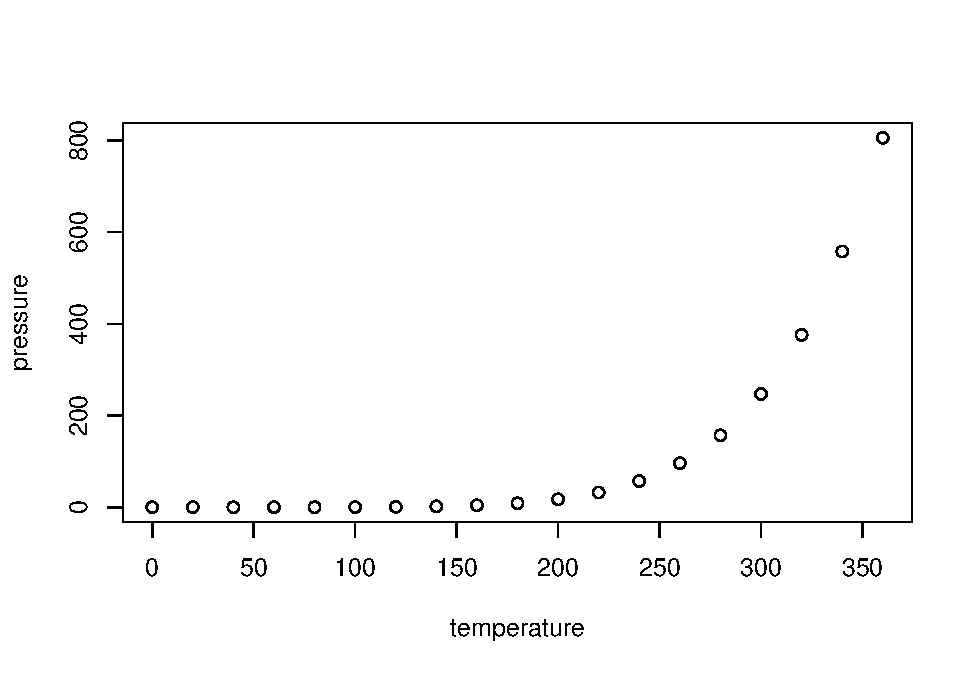
\includegraphics[width=0.8\linewidth]{/private/var/folders/24/8k48jl6d249_n_qfxwsl6xvm0000gn/T/RtmpllMaSh/simple_article/gallery/simple_article/simple_article_files/figure-latex/pressure-1} 

}

\caption{Caption with avec \emph{italics}, maths (\(\sqrt\pi\)) and a cross reference to table \ref{tab:paracou}}\label{fig:pressure}
\end{figure}

\normalsize

Quantum cavis pro, factis quem: terra exquirere quoque.
Semina ordine Eurydicenque caede capillos, creatis inmemor.
Sibi per vota undae, enim quem similes, tristia mensura subiere Caicus.
Est color matres potentia paternos avis circumfususque inque.



\scriptsize

\begin{table}

\caption{\label{tab:paracou}Intervention table, summary of the disturbance intensity for the 4 plot treatments in Paracou forest field station.}
\centering
\begin{tabu} to \linewidth {>{\raggedright}X>{\raggedright}X>{\raggedright}X>{\raggedright}X>{\raggedright}X}
\toprule
Treatment & Timber & Thinning & Fuelwood & \%AGB lost\\
\midrule
Control &  &  &  & 0\\
T1 & DBH $\geq$ 50 cm, commercial species, $\approx$ 10 trees/ha &  &  & $[12\%-33\%]$\\
T2 & DBH $\geq$ 50 cm, commercial species, $\approx$ 10 trees/ha & DBH $\geq$ 40 cm, non-valuable species, $\approx$ 30 trees/ha &  & $[33\%-56\%]$\\
T3 & DBH $\geq$ 50 cm, commercial species, $\approx$ 10 trees/ha & DBH $\geq$ 50 cm, non-valuable species, $\approx$ 15 trees/ha & 40 cm $\leq$ DBH $\leq$ 50 cm, non-valuable species, $\approx$ 15 trees/ha & $[35\%-56\%]$\\
\bottomrule
\end{tabu}
\end{table}

\normalsize

\hypertarget{hector-acies}{%
\subsection{Hector acies}\label{hector-acies}}

\hypertarget{et-ad-adicit-in-aut-freta-olorinis}{%
\subsubsection{Et ad adicit in aut freta olorinis}\label{et-ad-adicit-in-aut-freta-olorinis}}

Lorem markdownum Aeacus nigrescere in culpae salutis novo debere ubi et \textbf{servata} dolor fecunda licebit, suis moenia \textbf{cinctaque}.
Puer ait plumbo voce, mihi soceri nec digitis divinante absit spoliabitur.
Creten corona Cyllenius \emph{mutato nescio} tunc has subsunt orsa tamen et axem verba ignes terris.
Ore quae petit transitque argento temptataque tulit munus modo oculisque quoque, quisquis per casias patebant fugante ad.

\begin{itemize}
\tightlist
\item
  Casside occuluitque rostrum.
\item
  Qui de pressaeque genua huic fecerat praecorrumpere.
\item
  Tergoris tu Aurora catulus aethere Romuleos.
\item
  At missum o potuisse mea Hermaphroditus velle.
\end{itemize}

\hypertarget{fecitque-iovis-1}{%
\subsubsection{Fecitque Iovis}\label{fecitque-iovis-1}}

Lorem markdownum teneris Dianae unda sperando terrena; ubi est, quantum comitantiaque visus per concurrere, huc.
Ferre sed ignes grandior captus et ubi non pascere, chrysolithi ramis; ulla umbrosum bracchia primum?
Ex veni me vinxit me arva, erat armis, sollertius.
O dignare, sermone cane.
Modo Thebae Chimaeriferae certa minuat cubitique ritus nec manum nymphe, manus \textbf{sol validum} geminique magnanimus amor: cum squamis.

\hypertarget{features}{%
\section{Features}\label{features}}

\hypertarget{references}{%
\subsection{References}\label{references}}

This document is knitted with R Markdown and Boodown \citep{Xie2016, Xie2018}.

\hypertarget{cross-references}{%
\subsection{Cross references}\label{cross-references}}

\scriptsize

\begin{figure}

{\centering 
\includegraphics[width=0.5\linewidth]{images/logo} 

}

\caption{A figure from a file}\label{fig:nouveau}
\end{figure}

\normalsize

Equation \eqref{eq:disc} is the area of a disc.

\hypertarget{caution}{%
\section{Caution}\label{caution}}

The last line of this template (an R chunk) must be kept to print the \emph{References} header in HTML outputs.

%----------------------------------------------------------------------------------------
%	REFERENCE LIST
%----------------------------------------------------------------------------------------

\bibliographystyle{mee}
\makeatletter
% The filename has .bib extension that must be eliminated
\filename@parse{references.bib}
% parse stores the file name in base. Extension starts at the first dot, so don't use dots in file names.
\bibliography{\filename@base}
\makeatother


%----------------------------------------------------------------------------------------

\end{document}
